\documentclass[12pt,]{article}
\usepackage[T1]{fontenc}
\usepackage{lmodern}
\usepackage{amssymb,amsmath}
\usepackage{ifxetex,ifluatex}
\usepackage{fixltx2e} % provides \textsubscript
% use upquote if available, for straight quotes in verbatim environments
\IfFileExists{upquote.sty}{\usepackage{upquote}}{}
\ifnum 0\ifxetex 1\fi\ifluatex 1\fi=0 % if pdftex
  \usepackage[utf8]{inputenc}
\else % if luatex or xelatex
  \ifxetex
    \usepackage{mathspec}
    \usepackage{xltxtra,xunicode}
  \else
    \usepackage{fontspec}
  \fi
  \defaultfontfeatures{Mapping=tex-text,Scale=MatchLowercase}
  \newcommand{\euro}{€}
\fi
% use microtype if available
\IfFileExists{microtype.sty}{\usepackage{microtype}}{}
\usepackage[margin=1in]{geometry}
\usepackage{graphicx}
% Redefine \includegraphics so that, unless explicit options are
% given, the image width will not exceed the width of the page.
% Images get their normal width if they fit onto the page, but
% are scaled down if they would overflow the margins.
\makeatletter
\def\ScaleIfNeeded{%
  \ifdim\Gin@nat@width>\linewidth
    \linewidth
  \else
    \Gin@nat@width
  \fi
}
\makeatother
\let\Oldincludegraphics\includegraphics
{%
 \catcode`\@=11\relax%
 \gdef\includegraphics{\@ifnextchar[{\Oldincludegraphics}{\Oldincludegraphics[width=\ScaleIfNeeded]}}%
}%
\ifxetex
  \usepackage[setpagesize=false, % page size defined by xetex
              unicode=false, % unicode breaks when used with xetex
              xetex]{hyperref}
\else
  \usepackage[unicode=true]{hyperref}
\fi
\hypersetup{breaklinks=true,
            bookmarks=true,
            pdfauthor={},
            pdftitle={},
            colorlinks=true,
            citecolor=blue,
            urlcolor=blue,
            linkcolor=magenta,
            pdfborder={0 0 0}}
\urlstyle{same}  % don't use monospace font for urls
\setlength{\parindent}{0pt}
\setlength{\parskip}{6pt plus 2pt minus 1pt}
\setlength{\emergencystretch}{3em}  % prevent overfull lines
\setcounter{secnumdepth}{0}

\author{}
\date{}
\usepackage{lineno}
\linenumbers
\usepackage{setspace}
\doublespacing

\begin{document}

\normalsize


\section{Supplementary Information: Do we need detailed demographic data
to forecast population responses to climate
change?}\label{supplementary-information-do-we-need-detailed-demographic-data-to-forecast-population-responses-to-climate-change}

\subsubsection{Andrew T. Tredennick and Peter B.
Adler}\label{andrew-t.-tredennick-and-peter-b.-adler}

\emph{Andrew T. Tredennick
(\href{mailto:atredenn@gmail.com}{\href{mailto:atredenn@gmail.com}{atredenn@gmail.com}}),
Department of Wildland Resources and the Ecology Center, Utah State
University, Logan, UT}

\emph{Peter B. Adler, Department of Wildland Resources and the Ecology
Center, Utah State University, Logan, UT}

\begin{figure}[htbp]
\centering
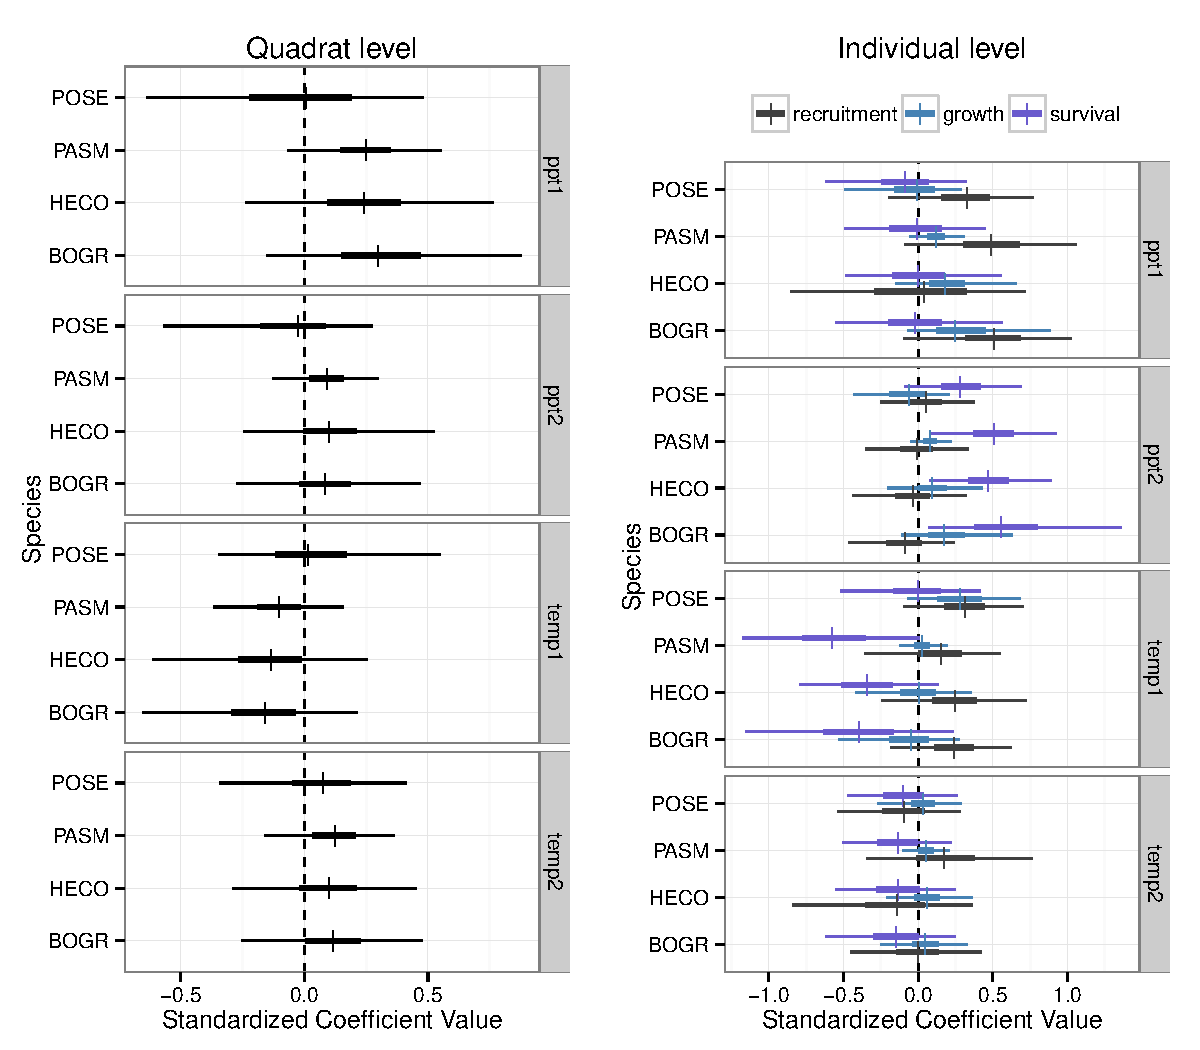
\includegraphics{components/figure/manuscript-figure_S1.pdf}
\caption{The proportion of interannual variability in vital rates
explained by the climate covariates. The contribution for growth is
defined as: (Climate model - Constant Model)/(Full model - Constant
model). The contribution for survival and colonization, where we could
not estimate a full model with year random effects at the quadrat level,
is defined as: (Constant Model - Climate Model)/Constant Model.}
\end{figure}

\begin{figure}[htbp]
\centering
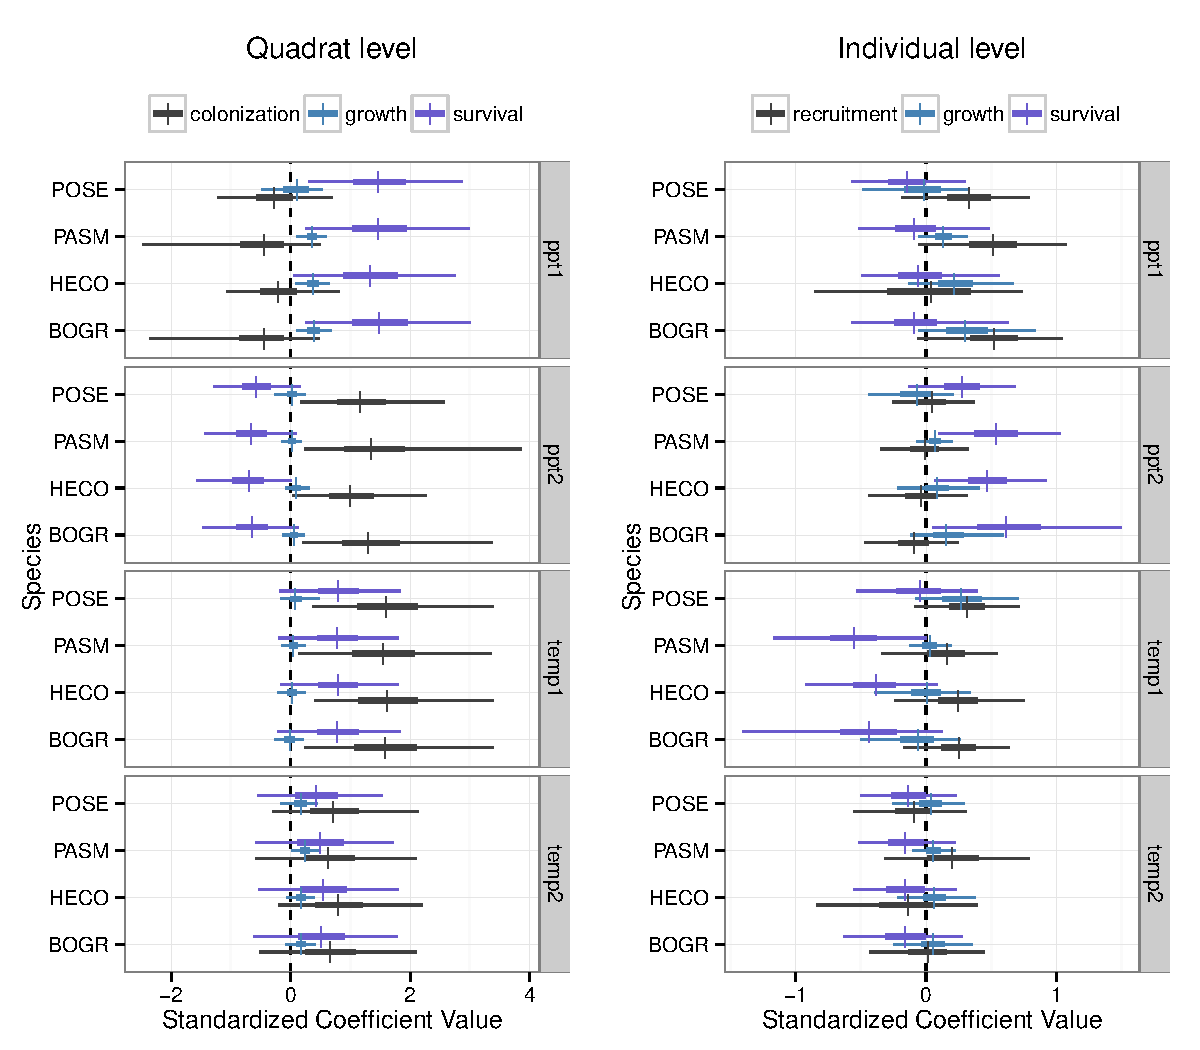
\includegraphics{components/figure/manuscript-figure_S2.pdf}
\caption{Posterior means (vertical ticks), 75\% credible intervals
(heavy lines), and 95\% credible intervals (light lines) of climate
effects on growth at both levels of inferences. The dashed vertical line
is at 0, indicating no effect.}
\end{figure}

\end{document}
